%You can leave alone everything before Line 79.
\documentclass{article}
\usepackage{url,amsfonts, amsmath, amssymb, amsthm,color, enumerate}
% Page layout
\setlength{\textheight}{8.75in}
\setlength{\columnsep}{2.0pc}
\setlength{\textwidth}{6.5in}
\setlength{\topmargin}{0in}
\setlength{\headheight}{0.0in}
\setlength{\headsep}{0.0in}
\setlength{\oddsidemargin}{0in}
\setlength{\evensidemargin}{0in}
\setlength{\parindent}{1pc}
\newcommand{\shortbar}{\begin{center}\rule{5ex}{0.1pt}\end{center}}
%\renewcommand{\baselinestretch}{1.1}
% Macros for course info
\newcommand{\courseNumber}{ME 552}
\newcommand{\courseTitle}{Mechatronics}
\newcommand{\semester}{Fall 2012}
\newcommand{\xxx}[1]{\textcolor{red}{#1}}
% Theorem-like structures are numbered within SECTION units
\theoremstyle{plain}
\newtheorem{theorem}{Theorem}[section]
\newtheorem{lemma}[theorem]{Lemma}
\newtheorem{corollary}[theorem]{Corollary}
\newtheorem{proposition}[theorem]{Proposition}
\newtheorem{statement}[theorem]{Statement}
\newtheorem{conjecture}[theorem]{Conjecture}
\newtheorem{fact}{Fact}
%definition style
\theoremstyle{definition}
\newtheorem{definition}[theorem]{Definition}
\newtheorem{example}{Example}
\newtheorem{problem}[theorem]{Problem}
\newtheorem{exercise}{Exercise}
\newtheorem{algorithm}{Algorithm}
%remark style
\theoremstyle{remark}
\newtheorem{remark}[theorem]{Remark}
\newtheorem{reduction}[theorem]{Reduction}
%\newtheorem{question}[theorem]{Question}
\newtheorem{question}{Question}
%\newtheorem{claim}[theorem]{Claim}
%
% Proof-making commands and environments
\newcommand{\beginproof}{\medskip\noindent{\bf Proof.~}}
\newcommand{\beginproofof}[1]{\medskip\noindent{\bf Proof of #1.~}}
\newcommand{\finishproof}{\hspace{0.2ex}\rule{1ex}{1ex}}
\def\therefore{\boldsymbol{\text{ }
\leavevmode
\lower0.4ex\hbox{$\cdot$}
\kern-.5em\raise0.7ex\hbox{$\cdot$}
\kern-0.55em\lower0.4ex\hbox{$\cdot$}
\thinspace\text{ }}}

\newenvironment{solution}[1]{\medskip\noindent{\bf Problem #1.~}}{\shortbar}

%====header======
\newcommand{\solutions}[4]{
%\renewcommand{\thetheorem}{{#2}.\arabic{theorem}}
\vspace{-2ex}
\begin{center}
{\small  \courseNumber, \courseTitle
\hfill {\Large \bf {#1} }\\
\semester, University of Michigan, Ann Arbor \hfill
{\em Date: #3}}\\
\vspace{-1ex}
\hrulefill\\
\vspace{4ex}
{\LARGE Lab Assignment #2}\\
\vspace{2ex}
\end{center}
\begin{trivlist}
\item \textsc{Team members:\\} {#4}
\end{trivlist}
\noindent
\shortbar
\vspace{3ex}
}
% math macros
\newcommand{\defeq}{\stackrel{\textrm{def}}{=}}
\newcommand{\Prob}{\textrm{Prob}}
%==
\usepackage{graphicx}
\usepackage{xfrac}
\begin{document}
%%%%%%%%%%%%%%%%%%%%%%%%%%%%%%%%%%%%%%%%%%%%%%%%%
%\solutions{Your name}{Problem Set Number}{Date of preparation}{Collaborators}{Prover}{Verifiers}
\solutions{}{2: MagLev}{\today}{Shiva Ghose, @gshiva\\ John Peterson, @jrpeters\\ Peter Turpel, @pturpel\\ Chan-Rong Lin, @pmelin}
%%%%%%%%%%%%%%%%%%%%%%%%%%%%%%%%%%%%%%%%%%%%%%%%%
%\renewcommand{\theproblem}{\arabic{problem}} 
%%%%%%%%%%%%%%%%%%%%%%%%%%%%%%%%%%%%%%%%%%%%%%%%%
%
% Begin the solution for each problem by
% \begin{solution}{Problem Number} and ends it with \end{solution}
%
% the solution for Problem 
\section*{Teamwork Participation Pledge :: Team 1}

I attest that I have made a fair and equitable contribution to this lab and submitted 
assignment. \\

My signature also indicates that I have followed the University of Michigan Honor Code, 
while working on this lab and assignment.\\

I accept my responsibility to look after all of the equipment assigned to me and my team, 
and that I have read and understood the X50 Lab Rules.\\

\begin{table}[h]
\begin{center}
    \begin{tabular}{|c|c|c|}
        \hline
        \textbf{Name} & \textbf{Email}     & \textbf{ \ \ \ \ \  \ \  \ \ \ \ \  \ \ Signature  \ \ \ \ \  \ \ \ \ \ \ \  \ \ } \\ \hline
        	~& ~& ~\\
	~& ~& ~\\
	Shiva Ghose   & gshiva@umich.edu   & ~                  \\
	~& ~& ~\\
	~& ~& ~\\ \hline 
	~& ~& ~\\
	~& ~& ~\\
        John Peterson & jrpeters@umich.edu & ~                  \\ 
	~& ~& ~\\
	~& ~& ~\\ \hline 
	~& ~& ~\\
	~& ~& ~\\
        Peter Turpel   & pturpel@umich.edu & ~                  \\
	~& ~& ~\\
	~& ~& ~\\ \hline 
	~& ~& ~\\
	~& ~& ~\\
        Chan-Rong Lin   & pmelin@umich.edu & ~                  \\
	~& ~& ~\\
	~& ~& ~\\ \hline 
        \hline
    \end{tabular}
\end{center}
\end{table}

\newpage

\section{Question 1}

\subsection*{a.}

\subsubsection{Break Beam Sensor}

\textbf{Assumptions} 
\begin{itemize}
\item Neglect Diffraction.
\item Light rays are parallel. 
\end{itemize}
As a consequence of these two assumptions the IR beam from the LED to the photo-transistor can be modeled as a cylinder.  The shadow casted by the sphere is then simply the circle with radius equal to the radius of the sphere.  This also means that the distance between the sphere and the IR LED does not matter, instead the only values that matter are the radius of the IR beam, the radius of the sphere, and the perpendicular distance between the axis of the beam and the center of the sphere.  The amount of light received by the photo-transistor can then simply be modeled as the intersection of two circles in 2-dimensions. \\

\[
  Radiance \hspace{0.1cm} Fraction = \left\{
  \begin{array}{l l}
    \frac{A_{beam} - A_{sphere}}{A_{beam}} & \quad \text{if } r_{sphere} + |d| < r_{beam} \\
    0 & \quad \text{if } r_{beam} + |d| < r_{sphere} \\
    1 & \quad \text{if } |d| < r_{beam} + r_{sphere} \\
    \frac{A_{beam} - A_{Overlap}}{A_{beam}} & \quad \text{if } |d| < r_{sphere} + r_{beam} \\
  \end{array} \right.
\]

\xxx{Format this part to look a bit nicer} \\
\textbf{Where:}
$$ A_{beam} = \pi r_{beam}^2 \hspace{1cm} A_{sphere} = \pi r_{sphere}^2 $$ 
$$ x = \frac{d^2+r_{beam}^2+r_{sphere}^2}{2d} \hspace{1cm} d_{beam}=x \hspace{1cm} d_{sphere}=d-x=\frac{d^2-r_{beam}^2+r_{sphere}^2}{2d} $$
$$ A_{Obeam} = r_{beam}^2 \cos^{-1} (\frac{d_{beam}}{r_{beam}})-d_{beam} \sqrt{r_{beam}^2-d_{beam}^2}$$ 
$$ A_{Osphere} = r_{sphere}^2 \cos^{-1} (\frac{d_{sphere}}{r_{sphere}})-d_{sphere} \sqrt{r_{sphere}^2-d_{sphere}^2}$$
$$ A_{Overlap} = A_{Obeam} + A_{Osphere} $$

\begin{figure}
\begin{center}
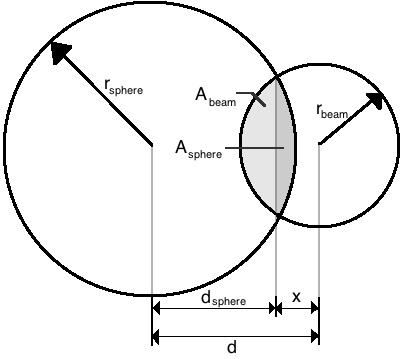
\includegraphics[width = 9cm]{beam_sphere_diagram.png}
\label{Q1_a1}
\caption{Planar approximation of IR beam occluded by steel sphere}
\end{center}
\end{figure}

\subsubsection{Driver Circuit}
\textbf{Assumptions}
\begin{itemize}
\item Op-Amp Golden Rules: voltage at inverting and non-inverting terminals is equal and op-amp input impedance is infinite
\end{itemize}

The electromagnet driver is a simple op-amp circuit, shown in figure \ref{Q1_a2}, which is designed to pass a specific current through the electromagnet for a a given input voltage.  The voltage at the non-inverting input can be simply determined by applying the voltage divider rule.  The voltage at the inverting input is now known allowing us to apply Ohm's Law to determine the current through $R_{3}$ and therefore through the electromagnet.  Notice that the resistance of the electromagnet does not affect the current provided by the driver circuit.

$$ V^{+}=\frac{R_2}{R_1+R_2}V_{in} \hspace{1cm} I_{EM}=\frac{V^{+}}{R_3}=\frac{1}{R_3}\left(\frac{R_2}{R_1+R_2}\right)V_{in} = DV_{in}$$

\begin{figure}
\begin{center}
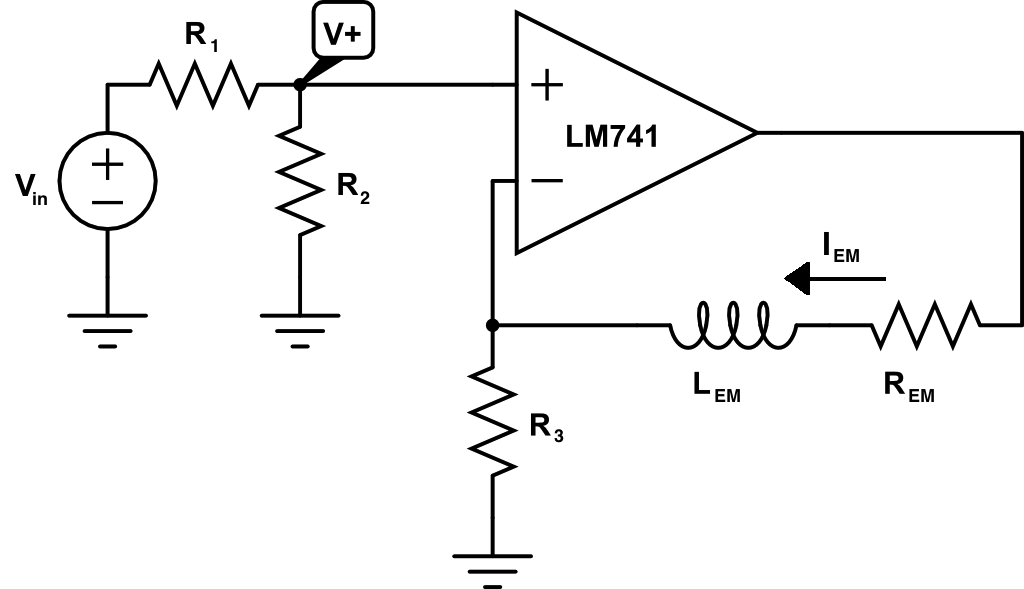
\includegraphics[width = 10cm]{em_driver_circuit.png}
\end{center}
\caption{Electromagnet Driver Circuit}
\label{Q1_a2}
\end{figure}

\subsubsection{Electro Magnet}
\textbf{Assumptions}
\begin{itemize}
\item $ \mu_{Al} \approx \mu_{Cu} \approx \mu_{air} $ 
\item $ \mu_{steel} \gg \mu_{air} $
\item can model the steel sphere as a cylinder with its axis collinear with the electromagnet  \\ 
$$A_{cd} \approx A_{s} = \pi * r_{sphere}^2 $$ 
\item neglect effects of fringing on cross-sectional area and assume particular dimensions of area of paths through the air that are consistent with the solid objects in the system \\
$$ A_{EM} = \pi*r_{EM}^2 \approx A_{ab} \hspace{1cm} A_{s} \approx A_{bc} \approx A_{de} \hspace{1cm} A_{EM} \approx A_{be} + A_{bc} $$ 
\item Path length from b to c does not vary with x: 
$ \frac{\partial}{\partial x} (L_{bc}) = 0$
\item The sphere remains in line with the axis of the electro magnet and $ x > 0$
\end{itemize}

Drawing out approximate flux paths yields the following diagram \xxx{make diagram of system} which can be converted to the following magnetic circuit shown in \ref{Q1_a3} by applying Ampere's Law and Maxwell's $2^{nd}$ law which yield the following three equations.  \\

\begin{figure}
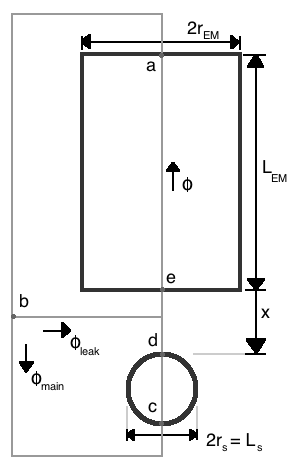
\includegraphics[width = 7cm]{flux_diagram.png}
\label{Q1_a3}
\caption{Approximate Flux paths taken through our system}
\end{figure}

$$ NI = \phi \left (\mathbb{R}_{EM} + \mathbb{R}_{ab}\right) + \phi_{main} \left( \mathbb{R}_{bc}+\mathbb{R}_{s}+\mathbb{R}_{dc} \right) $$
$$ NI = \phi \left( \mathbb{R}_{EM} + \mathbb{R}_{ab} \right) + \phi_{leak} \left( \mathbb{R}_{be} \right) $$
$$ \phi = \phi_{main} + \phi_{leak} $$


$$ \mathbb{R}_{EM} = \frac{L_{EM}}{A_{EM}\mu_{air}}  \hspace{1cm} \mathbb{R}_{ab} = \frac{L_{ab}}{A_{EM}\mu_{air}} \hspace{1cm} \mathbb{R}_{bc} = \frac{L_{bc}}{(A_{s})\mu_{air}} \hspace{1cm} \mathbb{R}_{de} = \frac{x}{A_{A_{s}}\mu_{air}} \hspace{1cm} $$ $$ \mathbb{R}_{be} = \frac{L_{be}}{(A_{EM} - A_{s})\mu_{air}}  \hspace{1cm}  \mathbb{R}_{s} = \frac{2*r_{sphere}}{A_{s}\mu_{steel}} \approx 0$$

Solving the $2^{nd}$ equation for $\phi_{leak}$ gives:

$$\phi_{leak} = C_{0}\left( NI-C_{1}\phi_{main} \right)$$ 
$$C_{0} = \frac{\mu_{air} A_{EM} (A_{EM} - A_{s})}{L_{be} A_{EM} + (L_{EM} + L_{ab})(A_{EM} - A_{s}))} \hspace{1cm} 
C_{1} = \frac{L_{EM} + L_{ab}}{\mu_{air} A_{EM}} $$

Substituting back into the $1^{st}$ equation lets us solve for $\phi_{main}$ yielding: 

$$ \phi_{main} = \frac{NI(1-C_{0}C_{1})}{C_{1} - C_{0} C_{1}^2 + \frac{L_{bc}}{\mu_{air} A_{s}} + \frac{x}{\mu_{air} A_{s}}} $$

With equations for our fluxes we can now compute the self inductance and from that compute the force exerted on the steel sphere as a function of position and current.

$$ \lambda = N \phi = L(x) I $$
$$ W(i,x) = (\sfrac{1}{2}) L(x) I^2 = (\sfrac{1}{2}) N \phi(x) I =(\sfrac{1}{2}) N I (\phi_{main}(x) + \phi_{leak}(x))$$
$$ F(i,x) = \frac{d}{dx} (W(i,x) )= (\sfrac{1}{2}) N I ( \frac{d}{dx} (\phi_{main}) + \frac{d}{dx} (\phi_{leak})) $$

$$ \frac{d}{dx}(\phi_{main}) = - \frac{N I (1 - C_{0}C_{1} \mu_{air} A_{s}}{(\mu_{air} A_{s}(C_{1} - C_{0} C_{1}^2 + C_{2}) + x)^2} dx$$

$$ \frac{d}{dx}(\phi_{leak}) = -C_{0} C_{1} \frac{d}{dx}(\phi_{main})$$

Putting this pair of terms together yields our final expression for the force.

$$ F_{EM}(x) = -\frac{1}{2} \left( 1 - C_{0}C_{1} \right)^2 \frac{\mu_{air} A_{s} N^2 }{(\mu_{air} A_{s}(C_{1} - C_{0} C_{1}^2 + C_{2}) + x)^2} I^2 $$

We can then condense these terms to arrive at a simple equation to model the force, shown below.  Where values for A and B can be obtained experimentally.

$$ F_{EM}(x) = -\frac{A I^2}{(B+x)^2} $$

\subsubsection{Steel Sphere \& Magnet System}
\textbf{Assumptions}
\begin{itemize}
\item neglect air resistance.
\item Steel sphere does not collide with the magnet: $x > 0$
\end{itemize}

According to Newton's second law the sum of the forces on an object is proportional to the acceleration of the object.  After constructing a free body diagram of our system shown in \xxx{make free body diagram} we can very easily derive a model of the motion of our system.

$$ \sum F_x = mg + F_{EM} = mg -\frac{A I^2}{(B+x)^2} = m  \ddot{x}$$

\begin{figure}
\begin{center}
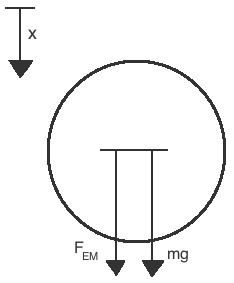
\includegraphics[width = 5cm]{freebodydiagram.png}
\label{Q1_a4}
\caption{Free body diagram of steel sphere.  Note: The x axis points downwards and our force was computed according to this convention, which is why their is a negative sign in the expression of the force generated by the electromagnet.}
\end{center}
\end{figure}

\subsection*{b.}
\subsubsection{Break Beam Sensor}

\subsubsection{Electromagnet \& Steel Sphere}
\xxx{Linearization goes here shiva}

\subsection*{c.}

\subsection*{d. Parameter Identification}

\subsubsection{Break Beam Sensor}
\xxx{how we acquired data, used shims and had the sphere on the stand, changed the height by known amounts and measured voltages}
\xxx{sensor data that we acquired plotted with our theoretical results based purely on the dimensions}
\xxx{plot of fitting rbeam to the data and plot the fitted result}
\xxx{refit this data, try to fit both rbeam and rblock to the optimal result}

\subsubsection{Driver Circuit}

Theoretically the conversion from voltage to current for this system should be very straight forwards.  We used a multi-meter to measure the resistances, noted in table \ref{Q1_dt1}, and then plugged these values into our model yielding the following relationship between current and input voltage.

$$ I_{EM Expected}=\frac{1}{R_3}\left(\frac{R_2}{R_1+R_2}\right)V_{in} = \frac{1}{0.5 \,\Omega}\left(\frac{999 \,\Omega}{42.3 \,k\Omega + 999 \,\Omega}\right)V_{in} = 0.04233 \, V_{in}$$

However examining the actual current and voltage relationship obtained by using the current measuring functionality of the multi-meter revealed that the above relationship did not hold.  Our observations showed a steady state current even when the input voltage was 0, so we fit a general linear model to the data excluding the input voltages above the current saturation.  It is also worth noting that we expected the electromagnet current to saturate at 510 mA rather than the 400 mA seen here.

$$ I_{EM Fit} = D \, V_{in} + C = 0.1781 \, V_{in} - 0.0179  \quad \textbf{if } V_{in} \leq 2.3 \, V $$

\begin{figure}
\begin{center}
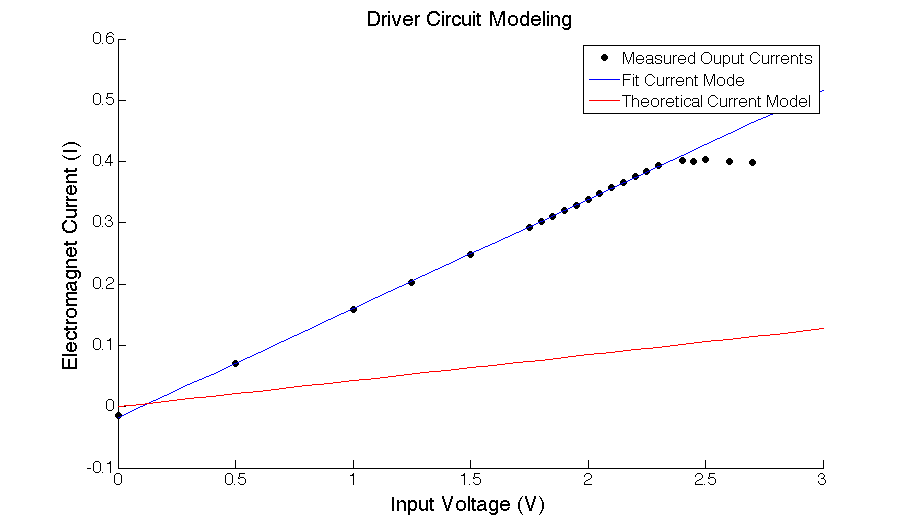
\includegraphics[width = 13cm]{DriverCircuitModel.png}
\label{Q1_d2}
\caption{Comparison of actual voltage current relationship with the fit model and the theoretical model}
\end{center}
\end{figure}

\begin{table}
\begin{center}
    \begin{tabular}{|c|c|}
        \hline
        Component & Resistance ($\Omega$) \\ \hline
        $R_{1}$   & 46200                 \\ 
        $R_{2}$   & 999                   \\ 
        $R_{3}$   & 0.5                   \\
        \hline
    \end{tabular}
\end{center}
\label{Q1_dt1}
\caption{Measured Resistances in driver circuit.}
\end{table}

\subsubsection{Electromagnet}
Examining our model for the force exerted by the electromagnet we see that we have two unknowns, A and B.  Now that we have a working system we were able to conduct an experiment where we levitated the sphere at various heights and measured the current associated with those heights.  We then attempted to perform non-linear optimization to determine A and B from this data however this computation diverged due to poor initial guesses for A and B.  To determine better initial guesses we symbolically solved for A and B as a function of two of these data points and then used these values as our initial estimate.  

$$ F(I,x) = \frac{A I^2}{(B+x)^2} $$
At equilibrium we know that the force exerted by the electromagnet must balance out the force of gravity on the sphere, this yields the following two expressions.
$$ mg = f = \frac{A I_{1}^2}{(B+x_{1})^2}  = \frac{A I_{2}^2}{(B+x_{2})^2} $$ 

We can solve the first expression for A.
$$ A = \frac{F (B + x_{1})^2}{I_{1}^2}$$

Then substituting the previous expression for A back into the $2^{nd}$ equation yields the following expression for B:
$$ B^2(1-R) + (2x_2-2x_1R)+x_2^2-x_1^2R = 0 \hspace{1cm} R = \frac{I_2^2}{I_1^1} $$

Choosing two of our x, I pairs allowed us to solve for plausible values of A and B which we used as initial guesses for the optimization allowing it to converge to the correct result.
\xxx{why are their two solutions? what is the physical reason, and which one makes sense as the right one}

\xxx{plot of actual data vs the fitted result}

\subsubsection{Steel Sphere}
\xxx{we just weighed it.}

\subsection*{e.}

\subsection*{f.}

\subsection*{g.}

\section{Part 2 Question 2}

\subsection*{a.}

\subsection*{b.}

\subsection*{c.}

\subsection*{d.}

\section*{Question 3}

\end{document}